% !TeX program = pdflatex
% !TeX encoding = UTF-8
% Documentation.tex

\documentclass[UTF8, oneside]{article}
\usepackage[a4paper, hmargin={1in, 1in}, vmargin={1in, 1in}]{geometry}
\usepackage{titlesec}
\usepackage[unicode,breaklinks]{hyperref}

\usepackage{amsmath}
\usepackage{amssymb}
\DeclareMathOperator{\arctantwo}{arctan2}
\usepackage{multicol}
\makeatletter
\newcommand*{\Rom}[1]{\expandafter\@slowromancap\romannumeral #1@}
\newcommand*{\rom}[1]{\expandafter\romannumeral #1@}
\makeatother

\usepackage{float}
\usepackage{sourcecodepro}
\usepackage{listings}
\lstset{
    frame=single,
    basicstyle=\sffamily
}
\usepackage{framed}
\usepackage{caption}
\usepackage{pdfpages}

\usepackage{graphicx}
\usepackage{tikz}
\usetikzlibrary{patterns}
\usetikzlibrary{shapes.geometric}
\usetikzlibrary{arrows.meta}
\usetikzlibrary{angles}

\usepackage{microtype}

\setlength\parskip{\baselineskip}

\title{Euler Angles}
\author{Shang Jiaxuan}
\date{\today}
\begin{document}
\maketitle

\begin{abstract}
Euler Angles, even rotations on their own, have many conventions.
Euler angles have different rotation orders, rotations have different
"handedness".

According to Shoemake 1994, there are $3\times 2\times 2\times 2=24$
possible conventions with given rotation "handedness".

This code implements all 24. 

The rotation matrix to euler method takes later Mike 2014 improvement.

The implementation for quaternion to euler, however is derived independently,
and provides all solutions in $SU(2)$ (keeping the sign of quaternion) or 
$SO(3)$.

The direct implementation takes less calculations and is potentially more
accurate.

After implementation, the formula is found to be equivalent to that of the
Evandro, Stéphane 2022 paper on similar matter.

This article aims to provide a detailed explanation of background and
implementation.
\end{abstract}


\section{Conventions}
There are occasions where many different terms can be commonly confused
and used interchangeably while they shouldn't. This section aims to clarify
those terms and establish a grounding for clear delivery.

\subsection{Matrix Storage}
When a matrix is stored in linear memory, the elements are normally tiled
either row first or column first. This does NOT affect what matrix it
represents, but is merely a choice of storage.

Similarly, one could choose to store a matrix in zig-zag order. This is
often the case for what Vulkan calls \texttt{VK\_IMAGE\_LAYOUT\_SHADER\_READ\_ONLY\_OPTIMAL}
for images since it optimizes memory contiguity for nearby reads.

The following is a diagram of $4\times 4$ matrices stored in row major and
column major in memory.

\begin{figure}[H]
\centering
\resizebox{0.8\textwidth}{!}{
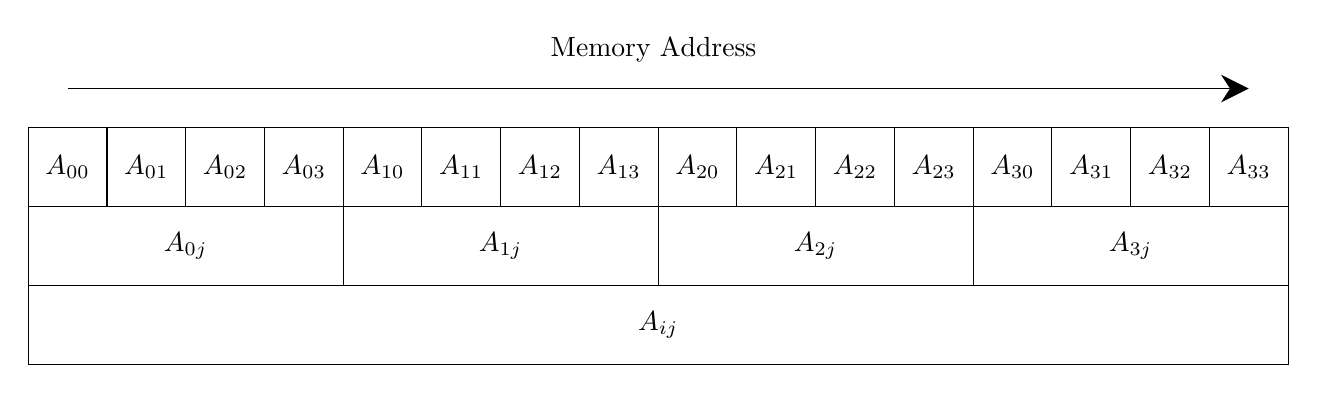
\begin{tikzpicture}
    \node[align=center] (mem) at (8, 4) { Memory Address };
    \draw[arrows = {-Stealth[width=10pt, length=10pt]}] (0.5, 3.5) -- (15.5, 3.5);
    \draw (0, 0) -- (16, 0) -- (16, 3) -- (0, 3) -- cycle;
    \draw (0, 1) -- (16, 1);
    \draw (0, 2) -- (16, 2);
    \draw (0, 3) -- (16, 3);
    \draw (1, 3) -- (1, 2);
    \draw (2, 3) -- (2, 2);
    \draw (3, 3) -- (3, 2);
    \draw (5, 3) -- (5, 2);
    \draw (6, 3) -- (6, 2);
    \draw (7, 3) -- (7, 2);
    \draw (9, 3) -- (9, 2);
    \draw (10, 3) -- (10, 2);
    \draw (11, 3) -- (11, 2);
    \draw (13, 3) -- (13, 2);
    \draw (14, 3) -- (14, 2);
    \draw (15, 3) -- (15, 2);
    \draw (4, 3) -- (4, 1);
    \draw (8, 3) -- (8, 1);
    \draw (12, 3) -- (12, 1);
    \node[align=center] (A) at (8, 0.5) {$A_{ij}$};
    \node[align=center] (A0) at (2, 1.5) {$A_{0j}$};
    \node[align=center] (A1) at (6, 1.5) {$A_{1j}$};
    \node[align=center] (A2) at (10, 1.5) {$A_{2j}$};
    \node[align=center] (A3) at (14, 1.5) {$A_{3j}$};
    \node[align=center] (A00) at (0.5, 2.5) {$A_{00}$};
    \node[align=center] (A01) at (1.5, 2.5) {$A_{01}$};
    \node[align=center] (A02) at (2.5, 2.5) {$A_{02}$};
    \node[align=center] (A03) at (3.5, 2.5) {$A_{03}$};
    \node[align=center] (A10) at (4.5, 2.5) {$A_{10}$};
    \node[align=center] (A11) at (5.5, 2.5) {$A_{11}$};
    \node[align=center] (A12) at (6.5, 2.5) {$A_{12}$};
    \node[align=center] (A13) at (7.5, 2.5) {$A_{13}$};
    \node[align=center] (A20) at (8.5, 2.5) {$A_{20}$};
    \node[align=center] (A21) at (9.5, 2.5) {$A_{21}$};
    \node[align=center] (A22) at (10.5, 2.5) {$A_{22}$};
    \node[align=center] (A23) at (11.5, 2.5) {$A_{23}$};
    \node[align=center] (A30) at (12.5, 2.5) {$A_{30}$};
    \node[align=center] (A31) at (13.5, 2.5) {$A_{31}$};
    \node[align=center] (A32) at (14.5, 2.5) {$A_{32}$};
    \node[align=center] (A33) at (15.5, 2.5) {$A_{33}$};
\end{tikzpicture}
}
\caption{Row Major Storage}
\label{row_major_storage}
\end{figure}
\begin{figure}[H]
\centering
\resizebox{0.8\textwidth}{!}{
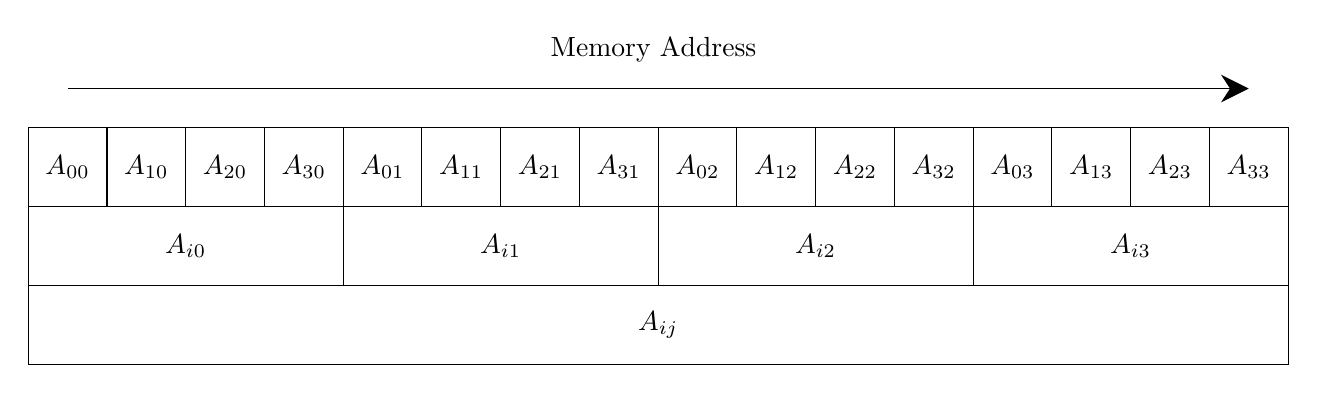
\begin{tikzpicture}
    \node[align=center] (mem) at (8, 4) { Memory Address };
    \draw[arrows = {-Stealth[width=10pt, length=10pt]}] (0.5, 3.5) -- (15.5, 3.5);
    \draw (0, 0) -- (16, 0) -- (16, 3) -- (0, 3) -- cycle;
    \draw (0, 1) -- (16, 1);
    \draw (0, 2) -- (16, 2);
    \draw (0, 3) -- (16, 3);
    \draw (1, 3) -- (1, 2);
    \draw (2, 3) -- (2, 2);
    \draw (3, 3) -- (3, 2);
    \draw (5, 3) -- (5, 2);
    \draw (6, 3) -- (6, 2);
    \draw (7, 3) -- (7, 2);
    \draw (9, 3) -- (9, 2);
    \draw (10, 3) -- (10, 2);
    \draw (11, 3) -- (11, 2);
    \draw (13, 3) -- (13, 2);
    \draw (14, 3) -- (14, 2);
    \draw (15, 3) -- (15, 2);
    \draw (4, 3) -- (4, 1);
    \draw (8, 3) -- (8, 1);
    \draw (12, 3) -- (12, 1);
    \node[align=center] (A) at (8, 0.5) {$A_{ij}$};
    \node[align=center] (Ax0) at (2, 1.5) {$A_{i0}$};
    \node[align=center] (Ax1) at (6, 1.5) {$A_{i1}$};
    \node[align=center] (Ax2) at (10, 1.5) {$A_{i2}$};
    \node[align=center] (Ax3) at (14, 1.5) {$A_{i3}$};
    \node[align=center] (A00) at (0.5, 2.5) {$A_{00}$};
    \node[align=center] (A10) at (1.5, 2.5) {$A_{10}$};
    \node[align=center] (A20) at (2.5, 2.5) {$A_{20}$};
    \node[align=center] (A30) at (3.5, 2.5) {$A_{30}$};
    \node[align=center] (A00) at (4.5, 2.5) {$A_{01}$};
    \node[align=center] (A10) at (5.5, 2.5) {$A_{11}$};
    \node[align=center] (A20) at (6.5, 2.5) {$A_{21}$};
    \node[align=center] (A30) at (7.5, 2.5) {$A_{31}$};
    \node[align=center] (A00) at (8.5, 2.5) {$A_{02}$};
    \node[align=center] (A10) at (9.5, 2.5) {$A_{12}$};
    \node[align=center] (A20) at (10.5, 2.5) {$A_{22}$};
    \node[align=center] (A30) at (11.5, 2.5) {$A_{32}$};
    \node[align=center] (A00) at (12.5, 2.5) {$A_{03}$};
    \node[align=center] (A10) at (13.5, 2.5) {$A_{13}$};
    \node[align=center] (A20) at (14.5, 2.5) {$A_{23}$};
    \node[align=center] (A30) at (15.5, 2.5) {$A_{33}$};
\end{tikzpicture}
}
\caption{Column Major Storage}
\label{column_major_storage}
\end{figure}

Memorywise, you can consider these to be transposed to each other, but
that only has meaning if you are doing memorywise "reinterpret\_cast" and
do not care about other possibilities.

\subsection{Vector Transforms}
In geometric libraries, we represent positions as vectors, while rotations and
other linear transformations as matrices. We can use column vectors, and multiply
matrices at the front. Or we can use row vectors and multiply matrices at the
right.

The relationship between the two is simple:

\begin{equation}
\begin{split}
v' &= Mv \\
v'^T &= (Mv)^T \\
&= v^T M^T
\end{split}
\end{equation}

Transformation matrices on row vectors are transposed compared to matrices on
column vectors. This includes translations and other matrices.

This is different from how one wants to store the matrix. One can make a matrix
composed of rows while using column vectors. The mismatch only matters if
one wishes to use SIMD, and using same row / column composition will result in
simple linear combinations while mismatch will mean memory contiguity for dot
products.

\subsection{Coordinate Handedness}
Although most of scientific work is done in right hand coordinates, there is
a major share of the graphics industry that uses left hand coordinate systems
so that when x axis goes to the right of screen, y axis goes up the screen, z
can point into the screen, which is the direction of view.

Different handedness of coordinate system means different sign of the Levi-Civita
Symbol, and a transposed rotation matrix.

But this does not change translation matrices to be in last row for column vector
transforms. Only rotations are affected.

\subsection{Rotations}
Rotations are not vectors. Angular speed is a pseudo-vector. Pseudo-vectors
behave differently in spatial inversions, and are actually shorthand for
tensors with the Levi-Civita Symbol.
\begin{equation}
\begin{split}
\mathbf{C} &= \mathbf{A}\times\mathbf{B}\\
P(\mathbf{C}) &= P(\mathbf{A})\times P(\mathbf{B})\\
&= (-\mathbf{A}) \times (-\mathbf{B})\\
&= \mathbf{C}
\end{split}
\end{equation}

Normally we would assign angular speed a direction according to the
"handedness" of the coordinate system.

\begin{figure}[hbt]
\centering
\resizebox{0.8\textwidth}{!}{
\begin{tikzpicture}
\draw[arrows = {-Stealth[width=5pt, length=5pt]}] (0, 0) -- (2, 0);
\draw[arrows = {-Stealth[width=5pt, length=5pt]}] (0, 0) -- (0, 2);
\draw[arrows = {-Stealth[width=5pt, length=5pt]}] (0, 0) -- (-1, -1);
\node (X) at (-1, -1.5) {$x$};
\node (Y) at (2.5, 0) {$y$};
\node (Z) at (0.5, 2) {$z$};
\begin{scope}[yscale=0.25]
\draw[arrows = {-Stealth[width=3pt, length=3pt]}] (0, 6) arc (-90:270:0.25); 
\end{scope}
\node[anchor=center, inner sep=0, rotate=90] (eye_along) at (0,-0.5)
    {\includegraphics[width=10pt]{eye.png}};
\node[anchor=south west] (along) at (0.5, -0.75) [font=\tiny]{Clockwise!};
\node[anchor=center, inner sep=0, rotate=270] (eye_reverse) at (0, 2.5)
    {\includegraphics[width=10pt]{eye.png}};
\node[anchor=south west] (reverse) at (0.5, 2.25) [font=\tiny]{Counter-Clockwise!};

\node[anchor=center, inner sep=0, yscale=-1] (thumb_left) at (-0.5, 1)
    {\includegraphics[width=12pt]{thumb_other.png}};
\node[anchor=south east] (reverse) at (-0.6, 1) [font=\tiny]{Negative!};
\node[anchor=center, inner sep=0, xscale=-1] (thumb_right) at (0.5, 0.875)
    {\includegraphics[width=10pt]{thumb.png}};
\node[anchor=south west] (reverse) at (0.5, 1) [font=\tiny]{Positive!};
\begin{scope}[yscale=0.25]
\draw[arrows = {-Stealth[width=3pt, length=3pt]}] (-0.5, 3.5) arc (-90:270:0.25);
\draw[arrows = {-Stealth[width=3pt, length=3pt]}] (0.5, 3.5) arc (-90:270:0.25); 
\end{scope}
\draw[arrows = {-Stealth[width=3pt, length=3pt]}] (-0.5, 0.9375) -- (-0.5, 0.4375);
\draw[arrows = {-Stealth[width=3pt, length=3pt]}] (0.5, 0.9375) -- (0.5, 1.4375);
\end{tikzpicture}
}
\caption{Direction of rotation}
\label{angle_direction}
\end{figure}


\subsection{Euler Order}
According to Shoemake 1994 article, there are only 2 fundamentally different euler angle
conventions: ones with repeating axis (Proper Euler Angles originally used by Euler), 
and ones without repeating axis (Tait Bryant Angles).

Proper Euler Angles have cleaner analytic formulas, whereas small Tait Bryant Angles can be
treated as small time delta of angular speed.

All conventions are either one combined with a permutation of axis order. The resulting
order will have two types of parity. This gives $3\times 2 \times 2$ possibilities.
Then one can choose the spinning axis, which reverses the first and last rotation.
Then the total is $3\times 2 \times 2\times 2 =24$ possibilities.

This library assigns the names of \texttt{roll->pitch->yaw} and
\texttt{bank->attitude->heading} to Tait Bryant Angles and 
\texttt{spin->nutation->precession} to Proper Euler Angles in rotation order
in static frame.
In the code, that is \texttt{rot0->rot1->rot2} in static frame or 
\texttt{rot2->rot1->rot0} in rotating frame.

This library encodes this metadata like this:
\begin{figure}[H]
\centering
\resizebox{0.8\textwidth}{!}{
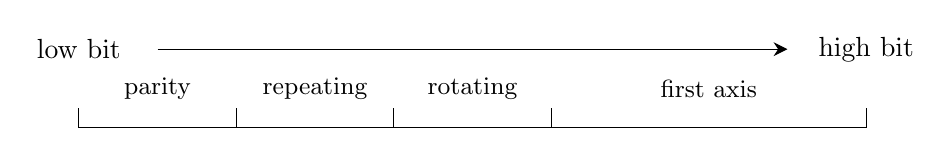
\begin{tikzpicture}
    \node[align=center] (low) at (0, 1) {\normalsize{low bit}};
    \node[align=center] (high) at (10, 1) {\normalsize{high bit}};
    \draw[arrows = {-Stealth[width=5pt, length=5pt]}] (1, 1) -- (9, 1);
    \draw (0, 0) -- (10, 0);
    \draw (0, 0) -- (0, 0.25);
    \node[align=center] (p) at (1, 0.5) {\small{parity}};
    \draw (2, 0) -- (2, 0.25);
    \node[align=center] (r) at (3, 0.5) {\small{repeating}};
    \draw (4, 0) -- (4, 0.25);
    \node[align=center] (rot) at (5, 0.5) {\small{rotating}};
    \draw (6, 0) -- (6, 0.25);
    \node[align=center] (a) at (8, 0.5) {\small{first axis}};
    \draw (10, 0) -- (10, 0.25);
\end{tikzpicture}
}
\caption{enum euler\_angle\_type encoding}
\end{figure}

This article will use $ijk$ notation when possible. $ij$ corresponds to $\theta_0, \theta_1$
axis, $k$ means $\theta_2$ axis for Tait-Bryant Angles. $k$ means the not-rotated axis in
Proper Euler Angles.

\subsection{Common Conventions}
Here is a non-comprehensive table of conventions for game engines and maths libraries.

\begin{table}[H]
\begin{center}
\begin{small}
\resizebox{\textwidth}{!}{
\begin{tabular}{p{5em}llllllp{6em}}
Library & Storage & Indexing & Vectors & Handed & Screen In & Rotation & Euler \\
\hline
this library & row & (row,col) & column & right & $-z$ & right hand & all \\
GLM / GLSL & column & [col][row] & column & right & $-z$ & right hand & Tait-Bryant \\
DirectXMath / HLSL & row & [row][col] & row & left & $+z$ & left hand & YXZs \\
Unity & column & [col][row] & column & left & $+z$ & left hand & ZXYs \\
Unreal & row & [row][col] & row & left & $-y$ & mixed & XYZs, XY right hand, Z left hand\\
Cocos & column & N/A & column & right & $-z$ & right hand & ZYXs \\
Ogre & row & [row][col] & column & right & $-z$ & right hand &  Tait-Bryant \\
CryEngine & row & [row][col] & column & right & $+y$ & right & ZYXs \\
CLHEP & row & [row][col] & column & right & N/A & left hand & ZYZs \\
Eigen & templated & (row,col) & N/A & N/A & N/A & N/A & N/A \\
\hline
\end{tabular}
}
\end{small}
\end{center}
\caption{Common Conventions}
\label{common_conventions}
\end{table}

This library's implementation of euler angles is NOT dependent on matrices being row major,
but relies on vectors being column vectors (matrices multiply on the left).

\section{Euler to Matrix/Quaternion}
As Shoemake's 1994 paper pointed out, there are only two matrices that matters:
\begin{align}
R_{ZYX} &= 
\begin{pmatrix}
\cos\theta_1\cos\theta_2 &
\sin\theta_1\sin\theta_0\cos\theta_2-\cos\theta_0\sin\theta_2 & 
\sin\theta_1\cos\theta_0\cos\theta_2+\sin\theta_0\sin\theta_2 \\
\cos\theta_1\sin\theta_2 &
\sin\theta_1\sin\theta_0\sin\theta_2+\cos\theta_0\cos\theta_2 &
\sin\theta_1\cos\theta_0\sin\theta_2-\sin\theta_0\cos\theta_2 \\
-\sin\theta_1 &
\cos\theta_1\sin\theta_0 &
\cos\theta_1\cos\theta_0
\end{pmatrix} 
\label{ZYX_matrix}\\
R_{XYX} &= 
\begin{pmatrix}
\cos\theta_1 &
\sin\theta_1\sin\theta_0 &
\sin\theta_1\cos\theta_0 \\
\sin\theta_1\sin\theta_2 &
-\cos\theta_1\sin\theta_0\sin\theta_2+\cos\theta_0\cos\theta_2 &
-\cos\theta_1\cos\theta_0\sin\theta_2-\sin\theta_0\cos\theta_2 \\
-\sin\theta_1\cos\theta_2 &
\cos\theta_1\sin\theta_0\cos\theta_2+\cos\theta_0\sin\theta_2 &
\cos\theta_1\cos\theta_0\cos\theta_2-\sin\theta_0\sin\theta_2
\end{pmatrix}
\label{XYX_matrix}
\end{align}

Similarly Quaternions have the formula:

\begin{align}
q_{ZYX}(wxyz) &=  
\begin{pmatrix}
q_0\\
q_i\\
q_j\\
q_k\\
\end{pmatrix}
&=&
\begin{pmatrix}
\cos\frac{\theta_1}{2}\cos\frac{\theta_0}{2}\cos\frac{\theta_2}{2} +
p\sin\frac{\theta_1}{2}\sin\frac{\theta_0}{2}\sin\frac{\theta_2}{2} \\
\cos\frac{\theta_1}{2}\sin\frac{\theta_0}{2}\cos\frac{\theta_2}{2} -
p\sin\frac{\theta_1}{2}\cos\frac{\theta_0}{2}\sin\frac{\theta_2}{2} \\
\sin\frac{\theta_1}{2}\cos\frac{\theta_0}{2}\cos\frac{\theta_2}{2} +
p\cos\frac{\theta_1}{2}\sin\frac{\theta_0}{2}\sin\frac{\theta_2}{2} \\
\cos\frac{\theta_1}{2}\cos\frac{\theta_0}{2}\sin\frac{\theta_2}{2} -
p\sin\frac{\theta_1}{2}\sin\frac{\theta_0}{2}\cos\frac{\theta_2}{2}
\end{pmatrix} \\
q_{XYX}(wxyz)  &= 
\begin{pmatrix}
q_0\\
q_i\\
q_j\\
q_k\\
\end{pmatrix}
&=&
\begin{pmatrix}
\cos\frac{\theta_1}{2}\cos(\frac{\theta_2}{2}+\frac{\theta_0}{2}) \\
\cos\frac{\theta_1}{2}\sin(\frac{\theta_2}{2}+\frac{\theta_0}{2}) \\
\sin\frac{\theta_1}{2}\cos(\frac{\theta_2}{2}-\frac{\theta_0}{2}) \\
p\sin\frac{\theta_1}{2}\sin(\frac{\theta_2}{2}-\frac{\theta_0}{2}) 
\end{pmatrix}
\end{align}

This is quite straight-forward.

Unit quaternion is a representations of $SU(2)$, whereas rotation matrix
(orthonormal $3\times 3$ matrix with $+1$ determinant) is a representation
of $SO(3)$.

$SU(2)$ double covers $SO(3)$, with $q$ and $-q$ mapping to the same rotation
matrix with $qvq^{-1}=M(q)v$.

The formulas have $2\pi$ period in $SO(3)$ (rotation matrix) whereas the period is
$4\pi$ in $SU(2)$ (quaternion).

This is very detailedly explained in differences of spin $\frac12$ spinors and
spin $1$ vectors.

\section{Matrix/Quaternion to Euler}

\subsection{Matrix (\texorpdfstring{$SO(3)$}{SO(3)}) to Euler}
When given a $3\times 3$ rotation matrix, there are actually normally two solutions for 
$\theta_0, \theta_1, \theta_2, \in [-\pi, +\pi]$. This can be shown by looking at the
rotation matrix. Proper Euler Angles only limits $\cos\theta_1$ whereas Tait Bryant Angles
only limits $\sin\theta_1$. This means one positive and one negative value possible
for the other trig function.

The normal convention for this is to make the other trig function of $\theta_1$ positive.
This gives a solution of Tait Bryant Angles for $\theta_1\in [-\frac\pi2, +\frac\pi2]$,
and a solution of Proper Euler Angles for $\theta_1\in [0, \pi]$.

If the solution for this convention is known, the other solution is
$\theta_0'=\pi-\theta_0$, $\theta_2'=\pi-\theta_2$, $\theta_1'=-\theta_1 (repeating)$
$\theta_1'=\pi-\theta_1 (non-repeating)$.

Shoemake's 1994 implementation of the general solution to solving euler angles from
rotation matrices is flawed by inverting the angles in the last step. This breaks the
solution choice for Proper Euler Angles if parity is different, giving 
$\theta_1\in [-\pi, 0]$.

This does not involve the so-called "Gimbal Lock" when the other trig function is $0$.

Mike Day's 2014 improvement on "Gimbal Lock" location can be summarized as such:

The euler angle matrix elements can be categorized into three categories. 1 Type \Rom{1}
element that is the single one with $\sin\theta_1$ or $\cos\theta_1$. 4 Type \Rom{2}
elements that are one term with the other trig function of $\theta_1$. 4 Type \Rom{3}
elements that are the most complicated, with two terms mixing everything.

Normally we use Type \Rom{1} element to calculate $\theta_1$, and then with the previously
said assumption, use Type \Rom{2} to calculate $\theta_0, \theta_2$. Type \Rom{3} elements are
discarded and only accessed on the special occasion of "Gimbal Lock".

When at "Gimbal Lock" Type \Rom{1} element goes to 1, Type \Rom{2} elements go to 0. Type \Rom{3}
elements stores all the information of the matrix when at "Gimbal Lock", giving the relation of
$\theta_0\pm\theta_2$, depending on the order of axis and which edge of the solution range it is on. 

The naive approach behaves badly at "Gimbal Lock" because Type \Rom{1} element $\approx 1-\frac12 \delta^2$.
Thus the error is approximately $\sqrt{2\mathtt{epsilon}}$. That is 3-4 digits for IEEE float.
Shoemake's original paper already takles this by using Type \Rom{2} elements to approximate
the other trig function, and improve $\theta_1$ value at "Gimbal Lock" via $\arctantwo$, 
giving $\theta_1$ with $\mathtt{epsilon}$ order error. But the behavior is still erratic by
requiring special treatment for "Gimbal Lock".

Mike's improvement is that Type \Rom{3} elements is used along with prior calculated
$\theta_0$ to give $\theta_2$. This automatically satisfies the relationship between
$\theta_0$ and $\theta_2$ at "Gimbal Lock" while being as continuous as possible for
all angles.

If the two Type \Rom{2} elements involving $\theta_2$ are used to give an estimate of
the other trig function of $\theta_1$, then all the elements of the $3\times 3$ matrix
are used to calculate the result. This gives a really good result.

This is what the implementation uses to calculate euler angles from matrices. Along with
adaptations to fix the flaw in Shoemake's method and using all elements to calculate.

For Proper Euler Angles:
\begin{equation}
\begin{split}
\sin\theta_1 &= \pm\sqrt{m_{ji}^2+m_{ki}^2}\\
\cos\theta_1 &= m_{ii} \\
\sin\theta_0 &= \frac{m_{ij}}{\sin\theta_1}\\
\cos\theta_0 &= p\frac{m_{ik}}{\sin\theta_1}\\
\sin\theta_2 &= p(m_{kj}\times\cos\theta_0-pm_{kk}\times\sin\theta_0) \\
\cos\theta_2 &= m_{jj}\times\cos\theta_0-pm_{jk}\times\sin\theta_0 
\end{split}
\end{equation}

\begin{equation}
\begin{split}
\sin\theta_1 >= 0 & \\
& \rightarrow \\
\theta_1 &= \arctantwo(\sqrt{m_{ji}^2+m_{ki}^2}, m_{ii})\\
\theta_0 &= \arctantwo(m_{ij}, pm_{ik}) \\
\theta_2 &= p\arctantwo(m_{kj}\times\cos\theta_0-pm_{kk}\times\sin\theta_0,
m_{jj}\times\cos\theta_0-pm_{jk}\times\sin\theta_0)
\end{split}
\end{equation}
\begin{equation}
\begin{split}
\sin\theta_1 <= 0 & \\
& \rightarrow \\
\theta_1 &= \arctantwo(-\sqrt{m_{ji}^2+m_{ki}^2}, m_{ii})\\
\theta_0 &= \arctantwo(-m_{ij}, -pm_{ik}) \\
\theta_2 &= p\arctantwo(-m_{kj}\times\cos\theta_0+pm_{kk}\times\sin\theta_0,
-m_{jj}\times\cos\theta_0+pm_{jk}\times\sin\theta_0)
\end{split}
\end{equation}


For Tait Bryant Angles:
\begin{equation}
\begin{split}
\sin\theta_1 &= -pm_{ki}\\
\cos\theta_1 &= \pm\sqrt{m_{ii}^2+m_{ji}^2} \\
\sin\theta_0 &= p\frac{m_{kj}}{\cos\theta_1}\\
\cos\theta_0 &= \frac{m_{kk}}{\cos\theta_1}\\
\sin\theta_2 &= p(-m_{ij}\times\cos\theta_0+pm_{ik}\times\sin\theta_0) \\
\cos\theta_2 &= m_{jj}\times\cos\theta_0-pm_{jk}\times\sin\theta_0
\end{split}
\end{equation}

\begin{equation}
\begin{split}
\cos\theta_1 >= 0 & \\
& \rightarrow \\
\theta_1 &= p\arctantwo(-m_{ki}, \sqrt{m_{ii}^2+m_{ji}^2})\\
\theta_0 &= p\arctantwo(m_{kj}, m_{kk}) \\
\theta_2 &= p\arctantwo(-m_{ij}\times\cos\theta_0+pm_{ik}\times\sin\theta_0,
m_{jj}\times\cos\theta_0-pm_{jk}\times\sin\theta_0)
\end{split}
\end{equation}
\begin{equation}
\begin{split}
\cos\theta_1 <= 0 & \\
& \rightarrow \\
\theta_1 &= p\arctantwo(-m_{ki}, -\sqrt{m_{ii}^2+m_{ji}^2})\\
\theta_0 &= p\arctantwo(-m_{kj}, -m_{kk}) \\
\theta_2 &= p\arctantwo(m_{ij}\times\cos\theta_0-pm_{ik}\times\sin\theta_0,
-m_{jj}\times\cos\theta_0+pm_{jk}\times\sin\theta_0)
\end{split}
\end{equation}

Another numerically stable method that doesn't require specially treating
"Gimbal Lock" is CERN CLHEP's method. But when tried out seemed to be less
accurate than this one.

That method uses the following relations:

For Proper Euler Angles:
\begin{equation}
\begin{split}
m_{jj}+m_{kk}&=+\cos(\theta_2+\theta_0)(1+\cos\theta_1)\\
m_{jj}-m_{kk}&=+\cos(\theta_2-\theta_0)(1-\cos\theta_1)\\
m_{kj}-m_{jk}&=+p\sin(\theta_2+\theta_0)(1+\cos\theta_1)\\
m_{kj}+m_{jk}&=+p\sin(\theta_2-\theta_0)(1-\cos\theta_1)\\
m_{ki}m_{ik}-m_{ji}m_{ij}&=-\cos(\theta_2-\theta_0)\sin^2\theta_1\\
m_{ki}m_{ik}+m_{ji}m_{ij}&=-\cos(\theta_2+\theta_0)\sin^2\theta_1\\
m_{ji}m_{ik}-m_{ki}m_{ij}&=+p\sin(\theta_2-\theta_0)\sin^2\theta_1\\
m_{ji}m_{ik}+m_{ki}m_{ij}&=+p\sin(\theta_2+\theta_0)\sin^2\theta_1
\end{split}
\end{equation}

For Tait Bryant Angles:

\begin{equation}
\begin{split}
m_{ij}-m_{jk}&=-p\sin(\theta_2-\theta_0)(1+p\sin\theta_1) \\
m_{ij}+m_{jk}&=-p\sin(\theta_2+\theta_0)(1-p\sin\theta_1) \\
m_{jj}-m_{ik}&=+\cos(\theta_2+\theta_0)(1-p\sin\theta_1) \\
m_{jj}+m_{ik}&=+\cos(\theta_2-\theta_0)(1+p\sin\theta_1) \\
m_{ii}m_{kk}-m_{kj}m_{ji}&=+\cos(\theta_2+\theta_0)\cos^2\theta_1 \\
m_{ii}m_{kk}+m_{kj}m_{ji}&=+\cos(\theta_2-\theta_0)\cos^2\theta_1 \\
m_{ji}m_{kk}-m_{kj}m_{ii}&=+p\sin(\theta_2-\theta_0)\cos^2\theta_1 \\
m_{ji}m_{kk}+m_{kj}m_{ii}&=+p\sin(\theta_2+\theta_0)\cos^2\theta_1
\end{split}
\end{equation}

\subsection{Quaternion (\texorpdfstring{$SU(2)$}{SU(2)}) to Euler}
There are a total of 4 solution of $\theta_1$ in the $\theta_1$ period
$[-2\pi, +2\pi]$. $\theta_0, \theta_2$ range is elaborated later.

For Proper Euler Angles:
\begin{align*}
q_0 &=\cos\frac{\theta_1}{2}\cos(\frac{\theta_2}{2}+\frac{\theta_0}{2}) \\
q_i &=\cos\frac{\theta_1}{2}\sin(\frac{\theta_2}{2}+\frac{\theta_0}{2}) \\
q_j &=\sin\frac{\theta_1}{2}\cos(\frac{\theta_2}{2}-\frac{\theta_0}{2}) \\
q_k &=p\sin\frac{\theta_1}{2}\sin(\frac{\theta_2}{2}-\frac{\theta_0}{2})
\end{align*}
\begin{equation}
\begin{split}    
\cos^2\frac{\theta_1}{2} &= q_0^2+q_i^2 \\
\sin^2\frac{\theta_1}{2} &= q_j^2+q_k^2 \\
\cos(\frac{\theta_2}{2}+\frac{\theta_0}{2}) &= \frac{q_0}{\cos\frac{\theta_1}{2}} \\
\sin(\frac{\theta_2}{2}+\frac{\theta_0}{2}) &= \frac{q_i}{\cos\frac{\theta_1}{2}} \\
\cos(\frac{\theta_2}{2}-\frac{\theta_0}{2}) &= \frac{q_j}{\sin\frac{\theta_1}{2}} \\
\sin(\frac{\theta_2}{2}-\frac{\theta_0}{2}) &= p\frac{q_k}{\sin\frac{\theta_1}{2}}
\end{split}
\end{equation}
Solution 0:
\begin{equation}
\begin{split}    
\theta_1 \in [0, \pi]  &
\rightarrow \frac{\theta_1}{2} \in [0, \frac\pi2] \\
&\rightarrow 
\cos\frac{\theta_1}{2} \ge 0,\ \sin\frac{\theta_1}{2} \ge 0\\
\theta_1 &= 2\arctantwo(\sqrt{q_j^2+q_k^2}, \sqrt{q_0^2+q_i^2}) \\
\frac{\theta_0}{2}+\frac{\theta_2}{2} &= \arctantwo(q_i, q_0) \\
&= \alpha \\
\frac{\theta_0}{2}-\frac{\theta_2}{2} &= \arctantwo(pq_k, q_j) \\
&= \beta
\end{split}
\end{equation}
Solution 1:
\begin{equation}
\begin{split}    
\theta_1 \in [-\pi, 0]  &
\rightarrow \frac{\theta_1}{2} \in [-\frac\pi2, 0] \\
&\rightarrow 
\cos\frac{\theta_1}{2} \ge 0,\ \sin\frac{\theta_1}{2} \le 0\\
\theta_1 &= 2\arctantwo(-\sqrt{q_j^2+q_k^2}, \sqrt{q_0^2+q_i^2}) \\
\frac{\theta_0}{2}+\frac{\theta_2}{2} &= \arctantwo(q_i, q_0) \\
&= \alpha \\
\frac{\theta_0}{2}-\frac{\theta_2}{2} &= \arctantwo(-pq_k, -q_j) \\
&= \beta
\end{split}
\end{equation}
Solution 2:
\begin{equation}
\begin{split}    
\theta_1 \in [\pi, 2\pi]  &
\rightarrow \frac{\theta_1}{2} \in [\frac\pi2, \pi] \\
&\rightarrow 
\cos\frac{\theta_1}{2} \le 0,\ \sin\frac{\theta_1}{2} \ge 0\\
\theta_1 &= 2\arctantwo(\sqrt{q_j^2+q_k^2}, -\sqrt{q_0^2+q_i^2}) \\
\frac{\theta_0}{2}+\frac{\theta_2}{2} &= \arctantwo(-q_i, -q_0) \\
&= \alpha \\
\frac{\theta_0}{2}-\frac{\theta_2}{2} &= \arctantwo(pq_k, q_j) \\
&= \beta
\end{split}
\end{equation}
Solution 3:
\begin{equation}
\begin{split}    
\theta_1 \in [-2\pi, -\pi]  &
\rightarrow \frac{\theta_1}{2} \in [-\pi, -\frac\pi2] \\
&\rightarrow 
\cos\frac{\theta_1}{2} \le 0,\ \sin\frac{\theta_1}{2} \le 0\\
\theta_1 &= 2\arctantwo(-\sqrt{q_j^2+q_k^2}, -\sqrt{q_0^2+q_i^2}) \\
\frac{\theta_0}{2}+\frac{\theta_2}{2} &= \arctantwo(-q_i, -q_0) \\
&= \alpha \\
\frac{\theta_0}{2}-\frac{\theta_2}{2} &= \arctantwo(-pq_k, -q_j) \\
&= \beta
\end{split}
\end{equation}
\begin{equation}
\begin{split}    
\theta_0 &= \alpha + \beta \\
\theta_2 &= \alpha - \beta
\end{split}
\end{equation}
For Tait Bryant Angles:
\begin{align*}
q_0 &=\cos\frac{\theta_1}{2}\cos\frac{\theta_0}{2}\cos\frac{\theta_2}{2} +
p\sin\frac{\theta_1}{2}\sin\frac{\theta_0}{2}\sin\frac{\theta_2}{2} \\
q_i &=\cos\frac{\theta_1}{2}\sin\frac{\theta_0}{2}\cos\frac{\theta_2}{2} -
p\sin\frac{\theta_1}{2}\cos\frac{\theta_0}{2}\sin\frac{\theta_2}{2} \\
q_j &=\sin\frac{\theta_1}{2}\cos\frac{\theta_0}{2}\cos\frac{\theta_2}{2} +
p\cos\frac{\theta_1}{2}\sin\frac{\theta_0}{2}\sin\frac{\theta_2}{2} \\
q_k &=\cos\frac{\theta_1}{2}\cos\frac{\theta_0}{2}\sin\frac{\theta_2}{2} -
p\sin\frac{\theta_1}{2}\sin\frac{\theta_0}{2}\cos\frac{\theta_2}{2}
\end{align*}
\begin{equation}
\begin{split}
q_iq_k-pq_0q_j &= -p\sin\frac{\theta_1}{2}\cos\frac{\theta_1}{2} \\
q_iq_k+pq_0q_j &= 2\sin\frac{\theta_0}{2}\cos\frac{\theta_0}{2}
\sin\frac{\theta_2}{2}\cos\frac{\theta_2}{2} 
+p\sin\frac{\theta_1}{2}\cos\frac{\theta_1}{2}
\left(\cos^2\frac{\theta_0}{2}-\sin^2\frac{\theta_0}{2}\right)
\left(\cos^2\frac{\theta_2}{2}-\sin^2\frac{\theta_2}{2}\right) \\
q_0+q_j&=\left(\cos\frac{\theta_1}{2}+\sin\frac{\theta_1}{2}\right)
\left(\cos\frac{\theta_0}{2}\cos\frac{\theta_2}{2}
+p\sin\frac{\theta_0}{2}\sin\frac{\theta_2}{2}\right) \\
q_0-q_j&=\left(\cos\frac{\theta_1}{2}-\sin\frac{\theta_1}{2}\right)
\left(\cos\frac{\theta_0}{2}\cos\frac{\theta_2}{2}
-p\sin\frac{\theta_0}{2}\sin\frac{\theta_2}{2}\right) \\
q_i+pq_k&=\left(\cos\frac{\theta_1}{2}-\sin\frac{\theta_1}{2}\right)
\left(\sin\frac{\theta_0}{2}\cos\frac{\theta_2}{2}
+p\cos\frac{\theta_0}{2}\sin\frac{\theta_2}{2}\right) \\
q_i-pq_k&=\left(\cos\frac{\theta_1}{2}+\sin\frac{\theta_1}{2}\right)
\left(\sin\frac{\theta_0}{2}\cos\frac{\theta_2}{2}
-p\cos\frac{\theta_0}{2}\sin\frac{\theta_2}{2}\right)
\end{split}
\end{equation}
Taking parameters:
\begin{equation}
\begin{split}
f_{00} & = q_0+q_j \\
f_{01} & = q_0-q_j \\
f_{10} & = q_i-pq_k \\
f_{11} & = q_i+pq_k \\
A &= \cos\frac{\theta_1}{2}+\sin\frac{\theta_1}{2} \\
B &= \cos\frac{\theta_1}{2}-\sin\frac{\theta_1}{2} 
\end{split}
\end{equation}
We have:
\begin{equation}
\begin{split}
A^2 &=
f_{10}^2+f_{00}^2 \\
B^2 &=
f_{11}^2+f_{01}^2 \\
\sin\left(\frac{\theta_0}{2}+p\frac{\theta_2}{2}\right) &=
\frac{f_{11}}{B} \\
\cos\left(\frac{\theta_0}{2}+p\frac{\theta_2}{2}\right) &=
\frac{f_{01}}{B} \\
\sin\left(\frac{\theta_0}{2}-p\frac{\theta_2}{2}\right) &=
\frac{f_{10}}{A} \\
\cos\left(\frac{\theta_0}{2}-p\frac{\theta_2}{2}\right) &=
\frac{f_{00}}{A} \\
\sin\theta_1 &= 2(q_0q_j-q_iq_k) \\
\cos\theta_1 &= AB
\end{split}
\end{equation}
Solution 0:
\begin{equation}
\begin{split}
\theta_1 \in [-\frac\pi2, +\frac\pi2]  &
\rightarrow \frac{\theta_1}{2} \in [-\frac\pi4, +\frac\pi4] \\
&\rightarrow 
\cos\frac{\theta_1}{2} \ge |\sin\frac{\theta_1}{2}| \\
&\rightarrow A \ge 0, B \ge 0 \\
\theta_1 &= \arctantwo(2(q_0q_j-q_iq_k),\sqrt{\left(f_{11}^2+f_{01}^2\right)
\left(f_{10}^2+f_{00}^2\right)}) \\
\frac{\theta_0}{2}+p\frac{\theta_2}{2} &= \arctantwo(f_{11}, f_{01}) \\
&= \alpha \\
\frac{\theta_0}{2}-p\frac{\theta_2}{2} &= \arctantwo(f_{10}, f_{00}) \\
&= \beta
\end{split}
\end{equation}
Solution 1:
\begin{equation}
\begin{split}
\theta_1 & \in [-\pi, -\frac\pi2) \cup (+\frac\pi2, +\pi] \\
\sin\theta_1 &= 2(q_0q_j-q_iq_k) >= 0 \\
&\rightarrow \theta_1 \in (+\frac\pi2, +\pi] \\
&\rightarrow A > 0,  B < 0 \\
\theta_1 &= \arctantwo(2(q_0q_j-q_iq_k),-\sqrt{\left(f_{11}^2+f_{01}^2\right)
\left(f_{10}^2+f_{00}^2\right)}) \\
\frac{\theta_0}{2}+p\frac{\theta_2}{2} &= \arctantwo(-f_{11}, -f_{01}) \\
&= \alpha \\
\frac{\theta_0}{2}-p\frac{\theta_2}{2} &= \arctantwo(f_{10}, f_{00}) \\
&= \beta
\end{split}
\end{equation}
\begin{equation}
\begin{split}
\sin\theta_1 &= 2(q_0q_j-q_iq_k) <= 0 \\
&\rightarrow \theta_1 \in [-\pi, -\frac\pi2) \\
&\rightarrow A < 0,  B > 0 \\
\theta_1 &= \arctantwo(2(q_0q_j-q_iq_k),-\sqrt{\left(f_{11}^2+f_{01}^2\right)
\left(f_{10}^2+f_{00}^2\right)}) +  \\
\frac{\theta_0}{2}+p\frac{\theta_2}{2} &= \arctantwo(f_{11}, f_{01}) \\
&= \alpha \\
\frac{\theta_0}{2}-p\frac{\theta_2}{2} &= \arctantwo(-f_{10}, -f_{00}) \\
&= \beta
\end{split}
\end{equation}
Solution 2:
\begin{equation}
\begin{split}
\theta_1 & \in [-\frac{3\pi}2, -\pi) \cup (+\pi, +\frac{3\pi}2] \\
\sin\theta_1 &= 2(q_0q_j-q_iq_k) > 0 \\
&\rightarrow \theta_1 \in [-\frac{3\pi}2, -\pi) \\
&\rightarrow A < 0,  B \ge 0 \\
\theta_1 &= \arctantwo(2(q_0q_j-q_iq_k),-\sqrt{\left(f_{11}^2+f_{01}^2\right)
\left(f_{10}^2+f_{00}^2\right)}) - 2\pi \\
\frac{\theta_0}{2}+p\frac{\theta_2}{2} &= \arctantwo(f_{11}, f_{01}) \\
&= \alpha \\
\frac{\theta_0}{2}-p\frac{\theta_2}{2} &= \arctantwo(-f_{10}, -f_{00}) \\
&= \beta
\end{split}
\end{equation}
\begin{equation}
\begin{split}
\sin\theta_1 &= 2(q_0q_j-q_iq_k) < 0 \\
&\rightarrow \theta_1 \in (+\pi, +\frac{3\pi}2] \\
&\rightarrow A \ge 0,  B < 0 \\
\theta_1 &= \arctantwo(2(q_0q_j-q_iq_k),-\sqrt{\left(f_{11}^2+f_{01}^2\right)
\left(f_{10}^2+f_{00}^2\right)}) + 2\pi \\
\frac{\theta_0}{2}+p\frac{\theta_2}{2} &= \arctantwo(-f_{11}, -f_{01}) \\
&= \alpha \\
\frac{\theta_0}{2}-p\frac{\theta_2}{2} &= \arctantwo(f_{10}, f_{00}) \\
&= \beta
\end{split}
\end{equation}
Solution 3:
\begin{equation}
\begin{split}
\theta_1 & \in [-2\pi, -\frac{3\pi}2) \cup (+\frac{3\pi}2, +2\pi] \\
\sin\theta_1 &= 2(q_0q_j-q_iq_k) \ge 0 \\
&\rightarrow \theta_1 \in [-2\pi, -\frac{3\pi}2) \\
&\rightarrow A < 0,  B < 0 \\
\theta_1 &= \arctantwo(2(q_0q_j-q_iq_k),\sqrt{\left(f_{11}^2+f_{01}^2\right)
\left(f_{10}^2+f_{00}^2\right)}) - 2\pi \\
\frac{\theta_0}{2}+p\frac{\theta_2}{2} &= \arctantwo(-f_{11}, -f_{01}) \\
&= \alpha \\
\frac{\theta_0}{2}-p\frac{\theta_2}{2} &= \arctantwo(-f_{10}, -f_{00}) \\
&= \beta
\end{split}
\end{equation}
\begin{equation}
\begin{split}
\sin\theta_1 &= 2(q_0q_j-q_iq_k) \le 0 \\
&\rightarrow \theta_1 \in (+\frac{3\pi}2, +2\pi] \\
&\rightarrow A < 0,  B < 0 \\
\theta_1 &= \arctantwo(2(q_0q_j-q_iq_k),\sqrt{\left(f_{11}^2+f_{01}^2\right)
\left(f_{10}^2+f_{00}^2\right)}) + 2\pi \\
\frac{\theta_0}{2}+p\frac{\theta_2}{2} &= \arctantwo(-f_{11}, -f_{01}) \\
&= \alpha \\
\frac{\theta_0}{2}-p\frac{\theta_2}{2} &= \arctantwo(-f_{10}, -f_{00}) \\
&= \beta
\end{split}
\end{equation}
\begin{equation}
\begin{split}
\theta_0 &= \alpha + \beta \\
\theta_2 &= p(\alpha - \beta)
\end{split}
\end{equation}

The solutions do not need extra work on "Gimbal Lock" either, since they work
in relations of $\frac{\theta_0}{2}\pm\frac{\theta_2}{2}$. 

This direct quaternion to euler approach keeps the sign of quaternion, as
it works in $SU(2)$.

Additionally, this library allows specifying $\theta_1$ outside $[-2\pi, +\pi]$ range.
The convention for solution index is shown in figure \ref{euler_r1_index}:
\begin{figure}[H]
\centering
\resizebox{0.75\textwidth}{!}{
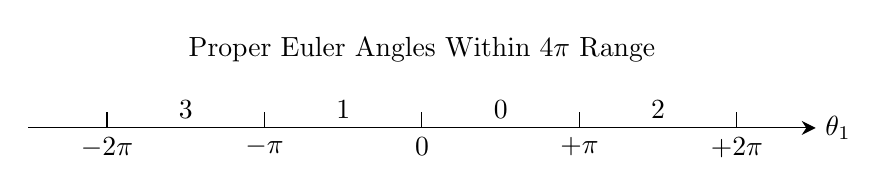
\begin{tikzpicture}
\node[align=center] (inside_proper) at (0, 1) {Proper Euler Angles Within $4\pi$ Range};
\draw[arrows = {-Stealth[width=5pt, length=5pt]}] (-5, 0) -- (5, 0) node[right] {$\theta_1$};
\draw (-4, 0.2) -- (-4, 0) node[below] {$-2\pi$};
\draw (-2, 0.2) -- (-2, 0) node[below] {$-\pi$};
\draw (0, 0.2) -- (0, 0) node[below] {$0$};
\draw (2, 0.2) -- (2, 0) node[below] {$+\pi$};
\draw (4, 0.2) -- (4, 0) node[below] {$+2\pi$};
\node[anchor=south] (r3) at (-3, 0) {$3$};
\node[anchor=south] (r1) at (-1, 0) {$1$};
\node[anchor=south] (r0) at (1, 0) {$0$};
\node[anchor=south] (r2) at (3, 0) {$2$};
\end{tikzpicture}
}
\resizebox{0.75\textwidth}{!}{
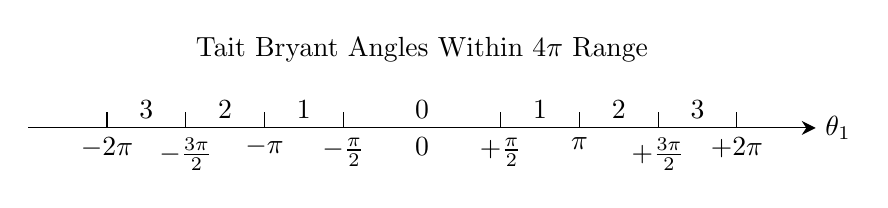
\begin{tikzpicture}
\node[align=center] (inside_proper) at (0, 1) {Tait Bryant Angles Within $4\pi$ Range};
\draw[arrows = {-Stealth[width=5pt, length=5pt]}] (-5, 0) -- (5, 0) node[right] {$\theta_1$};
\draw (-4, 0.2) -- (-4, 0) node[below] {$-2\pi$};
\draw (-3, 0.2) -- (-3, 0) node[below] {$-\frac{3\pi}{2}$};
\draw (-2, 0.2) -- (-2, 0) node[below] {$-\pi$};
\draw (-1, 0.2) -- (-1, 0) node[below] {$-\frac\pi2$};
\node[below] (origin) at (0, 0) {$0$};
\draw (1, 0.2) -- (1, 0) node[below] {$+\frac\pi2$};
\draw (2, 0.2) -- (2, 0) node[below] {$\pi$};
\draw (3, 0.2) -- (3, 0) node[below] {$+\frac{3\pi}{2}$};
\draw (4, 0.2) -- (4, 0) node[below] {$+2\pi$};
\node[anchor=south] (r0) at (0, 0) {$0$};
\node[anchor=south] (r1_0) at (1.5, 0) {$1$};
\node[anchor=south] (r1_1) at (-1.5, 0) {$1$};
\node[anchor=south] (r2_0) at (2.5, 0) {$2$};
\node[anchor=south] (r2_1) at (-2.5, 0) {$2$};
\node[anchor=south] (r3_0) at (3.5, 0) {$3$};
\node[anchor=south] (r3_1) at (-3.5, 0) {$3$};
\end{tikzpicture}
}
\resizebox{0.75\textwidth}{!}{
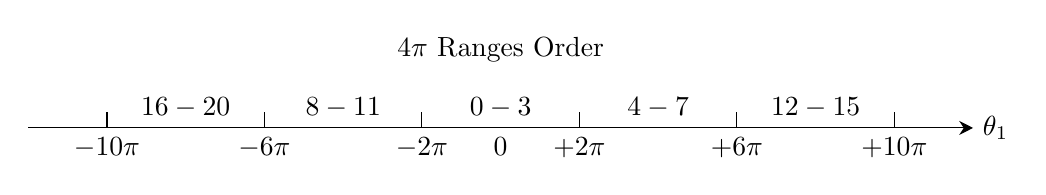
\begin{tikzpicture}
\node[align=center] (inside_proper) at (0, 1) {$4\pi$ Ranges Order};
\draw[arrows = {-Stealth[width=5pt, length=5pt]}] (-6, 0) -- (6, 0) node[right] {$\theta_1$};
\draw (-5, 0.2) -- (-5, 0) node[below] {$-10\pi$};
\draw (-3, 0.2) -- (-3, 0) node[below] {$-6\pi$};
\draw (-1, 0.2) -- (-1, 0) node[below] {$-2\pi$};
\node[below] (origin) at (0, 0) {$0$};
\draw (1, 0.2) -- (1, 0) node[below] {$+2\pi$};
\draw (3, 0.2) -- (3, 0) node[below] {$+6\pi$};
\draw (5, 0.2) -- (5, 0) node[below] {$+10\pi$};
\node[anchor=south] (r0) at (0, 0) {$0-3$};
\node[anchor=south] (r1) at (2, 0) {$4-7$};
\node[anchor=south] (r2) at (-2, 0) {$8-11$};
\node[anchor=south] (r3) at (4, 0) {$12-15$};
\node[anchor=south] (r4) at (-4, 0) {$16-20$};
\end{tikzpicture}
}
\caption{ $\theta_1$ Solution Index for $SU(2)$}
\label{euler_r1_index}
\end{figure}


The solutions of $\theta_0, \theta_2$ satisfies
$\frac{\theta_0}{2}\pm\frac{\theta_2}{2}\in [-\pi, +\pi]$.
This is a larger range than $\theta_0, \theta_2 \in [-\pi, +\pi]$, but smaller
range than $\theta_0, \theta_2 \in [-2\pi, +2\pi]$. As shown in figure \ref{r0r2_range}.

\begin{figure}[H]
\centering
\resizebox{0.75\textwidth}{!}{
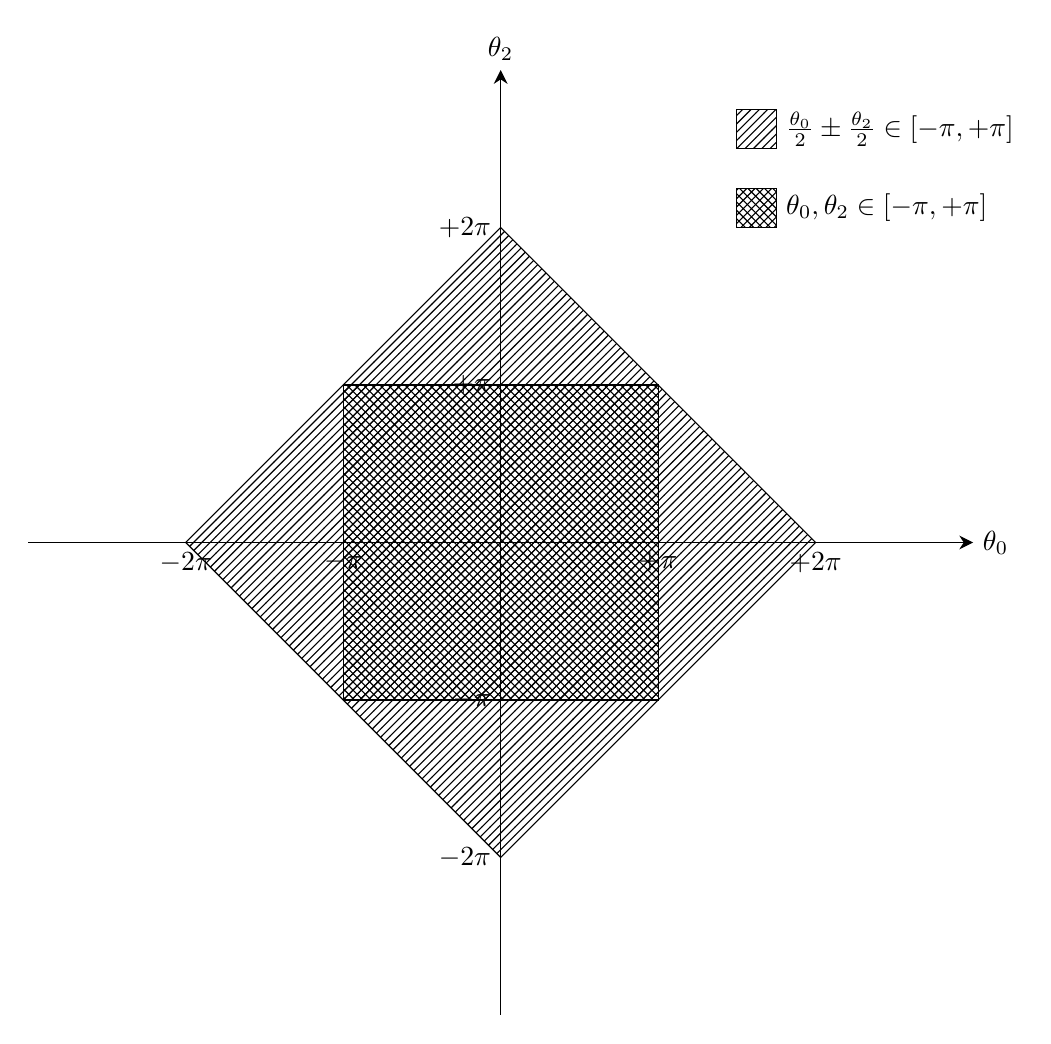
\begin{tikzpicture}
\draw[arrows = {-Stealth[width=5pt, length=5pt]}] (-6, 0) -- (6, 0) node[right]{$\theta_0$};
\draw[arrows = {-Stealth[width=5pt, length=5pt]}] (0, -6) -- (0, 6) node[above]{$\theta_2$};
\draw[pattern=crosshatch] (-2, -2) rectangle (2, 2);
\draw[pattern=north east lines] (-4, 0) -- (0, 4) -- (4, 0) -- (0, -4) -- cycle;
\node[anchor=north] (X_pi) at (2, 0) {$+\pi$};
\node[anchor=north] (X_2pi) at (4, 0) {$+2\pi$};
\node[anchor=north] (X_mpi) at (-2, 0) {$-\pi$};
\node[anchor=north] (X_m2pi) at (-4, 0) {$-2\pi$};
\node[anchor=east] (Y_pi) at (0, 2) {$+\pi$};
\node[anchor=east] (Y_2pi) at (0, 4) {$+2\pi$};
\node[anchor=east] (Y_mpi) at (0, -2) {$-\pi$};
\node[anchor=east] (Y_m2pi) at (0, -4) {$-2\pi$};

\draw[pattern=north east lines] (3, 5) rectangle (3.5, 5.5);
\draw[pattern=crosshatch] (3, 4) rectangle (3.5, 4.5);

\node[anchor=west] (legend_pm) at (3.5, 5.25)
    {$\frac{\theta_0}{2}\pm\frac{\theta_2}{2}\in[-\pi, +\pi]$};
\node[anchor=west] (legend_02) at (3.5, 4.25)
    {$\theta_0, \theta_2\in[-\pi, +\pi]$};
\end{tikzpicture}
}
\caption{Euler Angles $\theta_0, \theta_2$ from $SU(2)$ to $SO(3)$}
\label{r0r2_range}
\end{figure}

If one "corrects" one of $\theta_0, \theta_2$ if it lies outside the range 
$\theta_0, \theta_2 \in [-\pi, +\pi]$, one will get the result back to
single covering $SO(3)$, and inverting the quaternion in the process.

There is NO guarantee of having a SU(2) solution in
$\theta_0, \theta_1, \theta_2 \in [-\pi, +\pi]$ or $\theta_0, \theta_1, \theta_2 \in [0, 2\pi]$.


\end{document}
